\documentclass{article}

\usepackage{amsmath}
\usepackage{graphicx}
\usepackage{hyperref}

\usepackage[margin=0.6in]{geometry}

\title{Optimization Algorithm's from AI course}
\author{Filip Dabkowski}
\date{\today}

\begin{document}

\maketitle

\section{Objective}
Let's setup some objective to optimize as an example of usage. A common thing to optimize is fitting a line or more generally a function through some data.\newline

So first we need to get or generate some data. Like for example scores of students from Statistics exam, in relation to how much they like Statistics.
\begin{figure}[h]
    \centering
    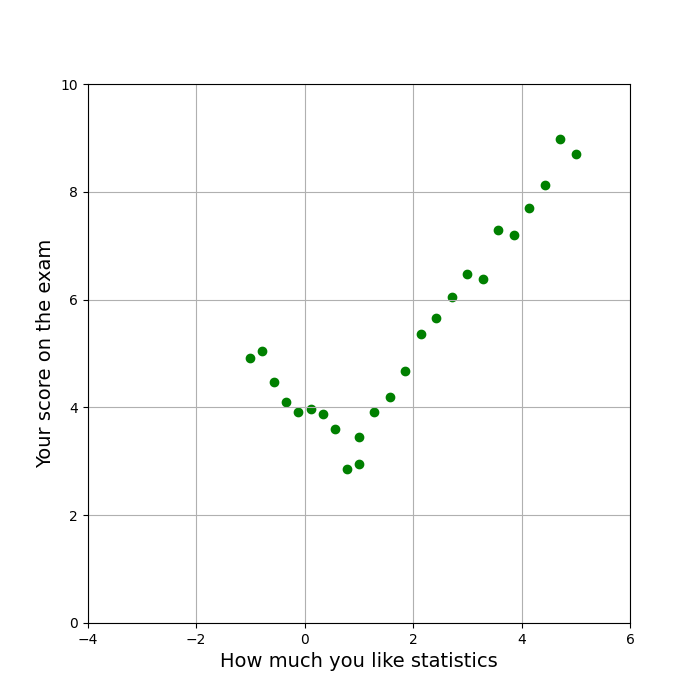
\includegraphics[width=0.4\textwidth]{../images/myplot.png}
    \caption{Example data}
    \label{fig:data}
\end{figure}

Now that we have our data, we can denote $x$ as measure of likeness and $y$ as grade of the student. In that case each point on our graph is $(x_i, y_i)$, where $i$ is number of student in the dataset.

\break

Lets begin with defining our function that is going to approximate the data, it could also be used later for making predictions. Like ''If your likeness of Statistics equals 4, you will probably get 7.74 on your final exam''

\begin{figure}[h]
    \centering
    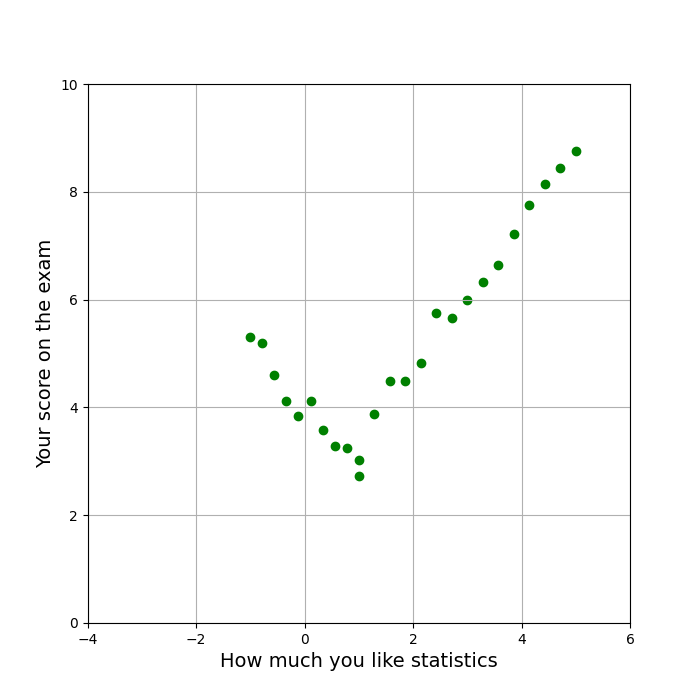
\includegraphics[width=0.4\textwidth]{../images/myplot1.png}
    \caption{Linear function $f(x) = 1 * x + 0$}
    \label{fig:data_line}
\end{figure}

Suppose our data can be approximated using a linear function, in our case it is not really true, however in real life we also can't visualize the whole dataset on a simple graph. Now we need some measure how well our model (function) fits the data (loss-function), so is it a good approximation or not. A common way to measure it, would be to calculate the squared difference between the actual value predicted value.

\begin{equation}
    \mathcal{L} = \sum_{i=1}^N{(y_i - f(x_i))^2}
\end{equation}

\textit{Side note, the loss function written above has a name (unfortunately more than one) Sum Squared Error (SSE), in ML circles it is more commonly know as L2 loss. It also has a more fancy notation, that you might find in papers... or YT videos.}

\begin{equation}
    L2 = || y - f(x) ||^2_2 = \sum_{i=1}^N{(y_i - f(x_i))^2}
\end{equation}

Now as you may see we have our loss-function that represent how badly our model preforms. If our loss were to reach 0 that would mean that the model perfectly fits the data. \textit{But how can we change our loss?} Of course by changing parameters in our model. The function $f(x) = 1 * x + 0$ has two parameters, currently set to $a=1$ and $b=0$, so our parametrized linear function is written as $f(x) = ax+b$. Now by changing parameters $a$ and $b$ we can lower or increase the loss. Now the expanded formula for the loss function is:

\begin{equation}
    \mathcal{L} = \sum_{i=1}^N{(y_i - (ax_i + b))^2}
\end{equation}

On the side note, the equation above is for the total loss, total since it is the sum of the loss of every point. More commonly used would be Mean Square Error (MSE) so basic average of the total loss.

\begin{equation}
    \mathcal{L} = \frac{1}{N}\sum_{i=1}^N{(y_i - (ax_i + b))^2}
\end{equation}

\section{Enumeration Method}
This is one of the simplest algorithms to understand, as the only thing that you need to do is to procedurally iterate through possible parameter values.\newline

The problem with that in our case is that possible values of the parameters $a$ and $b$ belong to real numbers. In math terms: $(a, b) \in \mathbf{R}\times\mathbf{R}$. So if we were to try plug in all the possible values for $a$ and $b$ we would be calculating forever with infinite precision. As a simplification we will only consider values in a range of $[-5,5]$ with step of $0.2$.

So now basically what we need to do is to alter both parameter's a little bit, changing our function and after each iteration of changing the parameter's, calculate the loss. We pick the pair of $a$ and $b$ parameter values that results in the smallest loss.

\begin{figure}[h]
    \centering
    \begin{minipage}{0.4\textwidth}
        \centering
        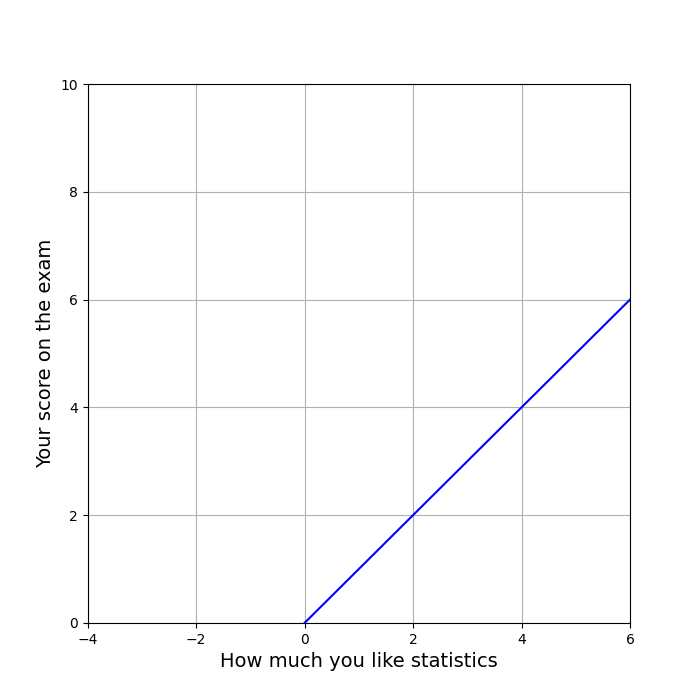
\includegraphics[width=\linewidth]{../images/myplot2.png}
        \caption{Altering the intercept parameter of our model}
    \end{minipage}
    \hfill
    \begin{minipage}{0.4\textwidth}
        \centering
        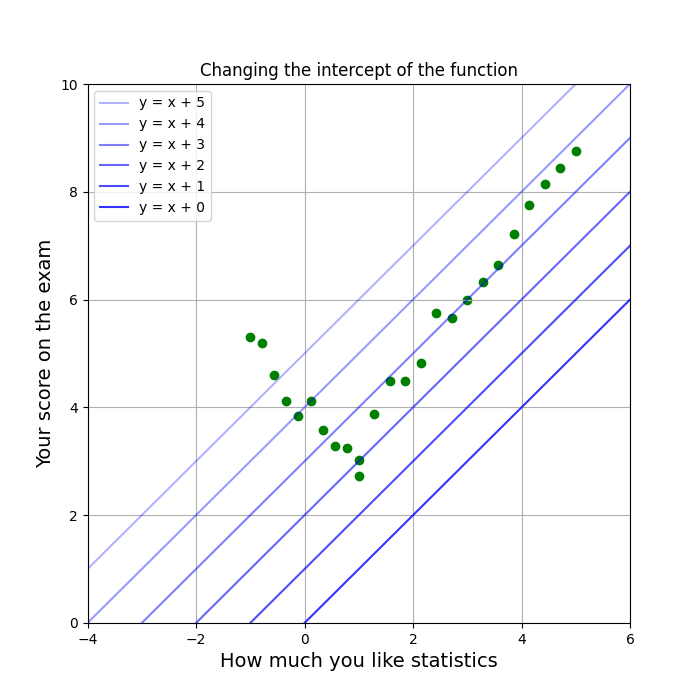
\includegraphics[width=\linewidth]{../images/myplot3.png}
        \caption{Altering the slope parameter of our model}
    \end{minipage}
\end{figure}

We not only tweak the parameter values on their own but also combinations of both of them. To visualize how the loss function depends on parameter values, here is a pretty plot.

\begin{figure}[h]
    \centering
    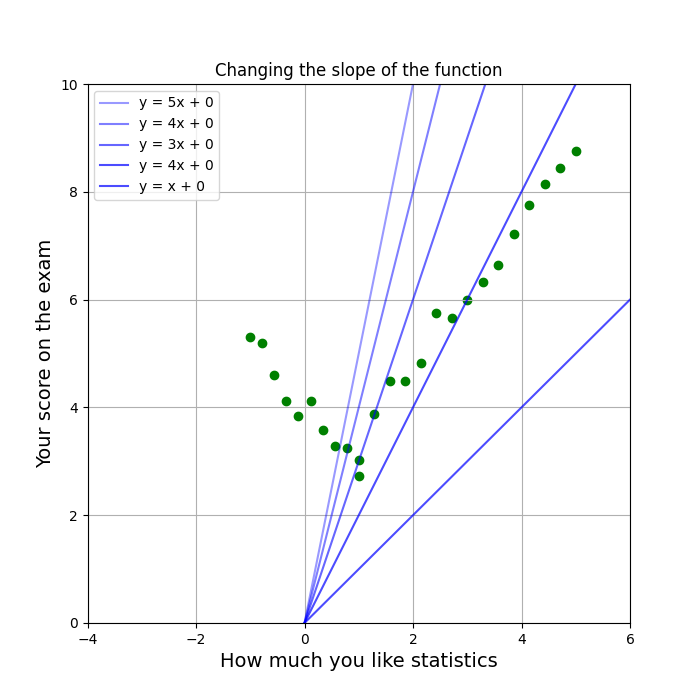
\includegraphics[width=0.66\textwidth]{../images/myplot4.png}
    \caption{Loss with respect to $a$ and $b$}
    \label{fig:loss_3d}
\end{figure}

\break

\section{Random Walking}

Remember how enumeration was structured checking of all possible values? Now with Random Walking, we take the same range of possible values but instead of all combinations, we pick a random number from each domain of possible values for $a$ and $b$ respectfully, and we check the loss at given random point. We do this $N$ times and pick the pair of $(a, b)$ values that results with the smallest loss.

\section{Random Search}

Random Search I believe was explained on the lectures quite well. Basic outline of this algorithm, Starting from a randomly sampled point $p = (a, b)$ we need to define initial range of searching $r$, from the point $p$ we sample another random point in the range $r$, new point is accepted and set as the current point if and only if the loss in new point is smaller.

\begin{figure}[h]
    \centering
    \begin{minipage}{0.4\textwidth}
        \centering
        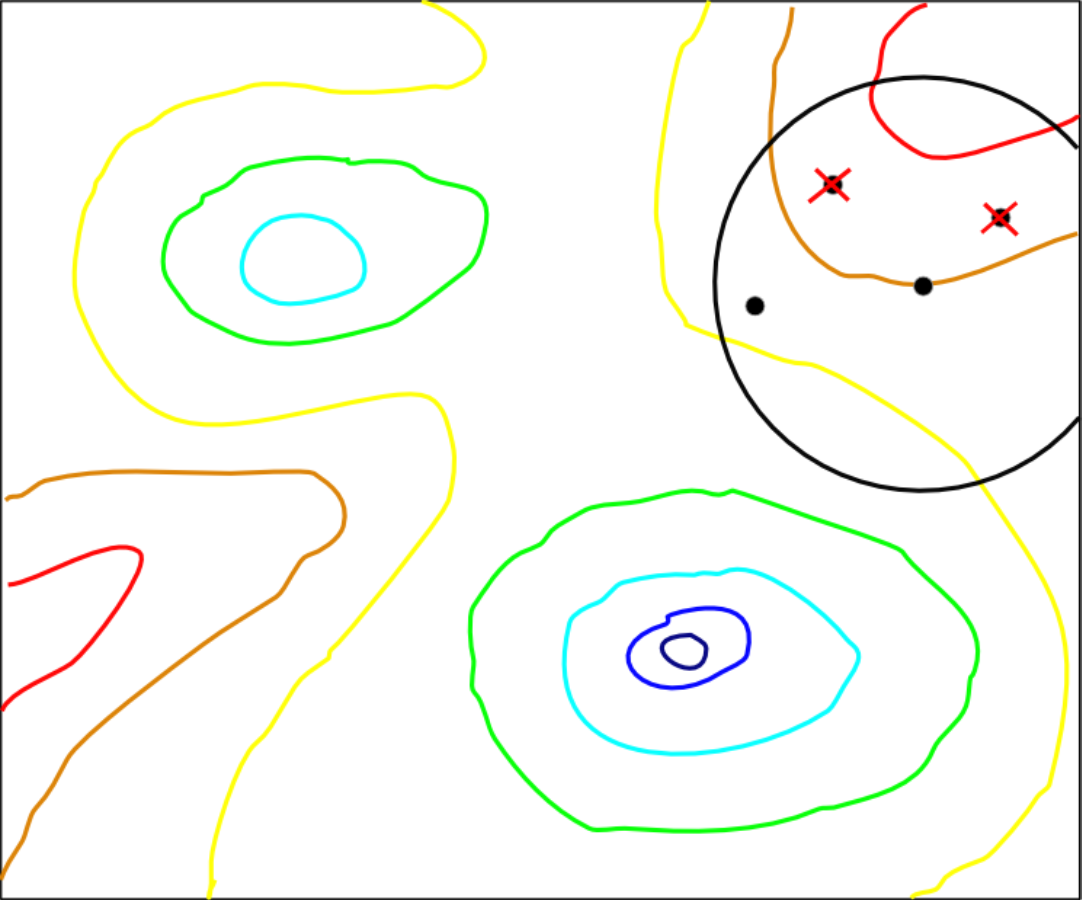
\includegraphics[width=\linewidth]{../images/screenshot1.png}
        \caption{Image from presentation, initial $p$ and few tries of new points.}
    \end{minipage}
    \hfill
    \begin{minipage}{0.4\textwidth}
        \centering
        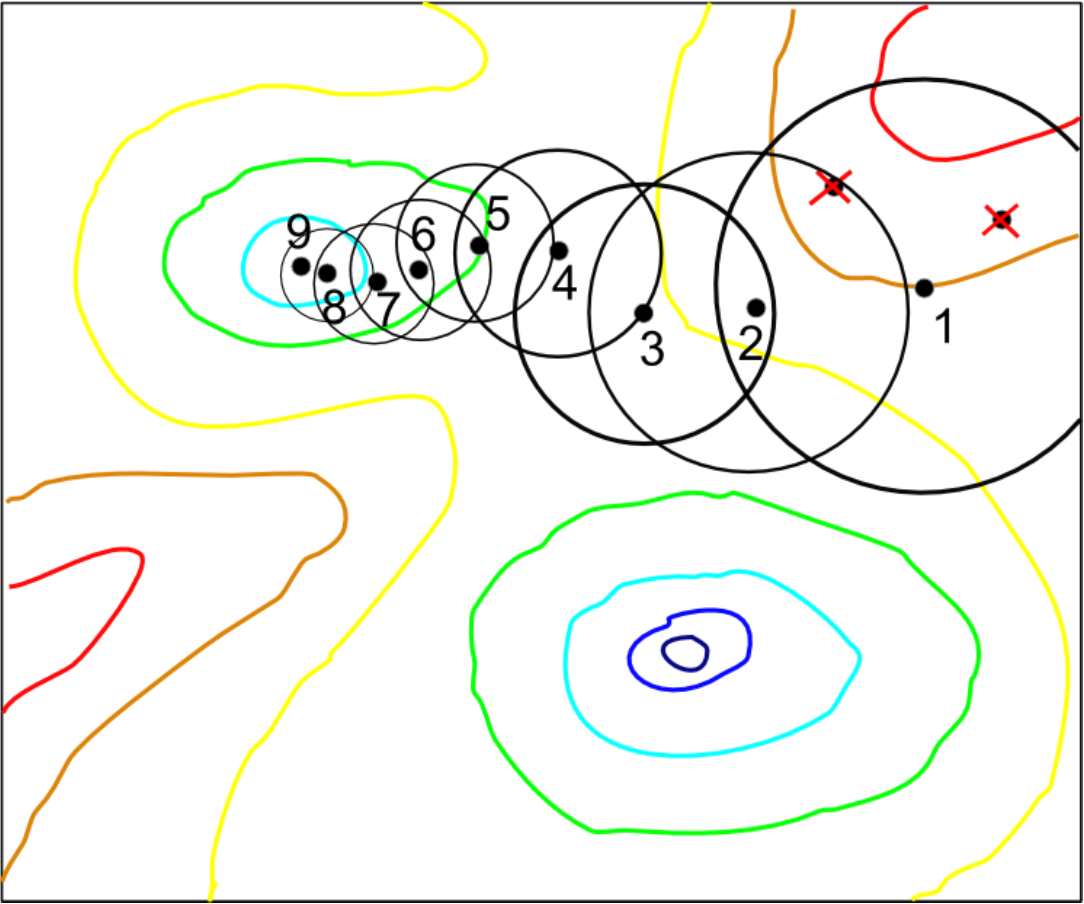
\includegraphics[width=\linewidth]{../images/screenshot2.png}
        \caption{Final state of the algorithm after many points have been sampled, notice how the range of search might be changing.}
    \end{minipage}
\end{figure}

\section{Simulated Annealing}

\section{Gradient Descent/Search}

This is the most commonly used method, especially when it comes to Neural Networks, however it is also the first one that requires us to have knowledge of the exact formula of the loss function. All the previous methods just 

\end{document}
